\documentclass[tikz, border=1mm]{standalone}
\usepackage{tikz} 
\usetikzlibrary{arrows.meta}
\usepackage{pgfplots}

\pgfplotsset{compat=1.18}

\begin{document}

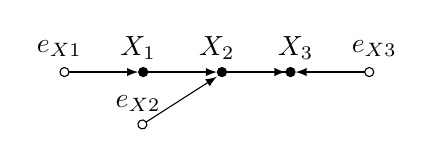
\begin{tikzpicture}

    % dag_bb3
    \node at (-2,0) {$e_{X1}$};
    \node at (-1,0) {$X_{1}$};
    \node at (-1,-0.7) {$e_{X2}$};
    \node at (0,0) {$X_{2}$};
    \node at (1,0) {$X_{3}$};
    \node at (2,0) {$e_{X3}$};

    \draw[{Circle[open]}-{latex}](-2,-0.3) to (-1,-0.3); % eX -> X (circle)
    \draw[{Circle}-{latex}](-1,-0.3) to (0,-0.3); % X -> Z
    \draw[{Circle[open]}-{latex}](-1,-1) to (0,-0.36); % eZ -> Z (circle)
    \draw[{Circle}-{latex}{Circle}](0,-0.3) to (1,-0.3); % Z -> Y
    \draw[{Circle[open]}-{latex}](2,-0.3) to (1,-0.3); % eY -> Y (circle)
    
\end{tikzpicture}

\end{document}
